%----------------------------------------------------------------------------
\chapter{Több kamerából álló kamera-rendszerek}
%----------------------------------------------------------------------------

Ebben a fejezetben a több kamerából álló rendszerekhez kapcsolódó különféle problémák, ezek megoldási lehetőségeiről lesz szó. A kitűzött feladat szempontjából két fontos részproblémát kell több kamerából álló rendszerek esetén megoldani. Az első ezek közül, hogy ha a kamerák nem egy közös feldolgozó egységhez kapcsolódnak, hanem például a kamerák képeit egy videófolyamként kapjuk, akkor szükséges lehet a folyamokat szinkronizálni. A második pedig, hogy a kamerák képei alapján a 3 dimenziós teret a lehető legjobban rekonstruáljuk.

\section{Kamerák szinkronizációja}

Az egyik lehetséges módszer a kamerák szinkronizációjára felhasználja, hogy a videófolyamba időpecséteket kódolunk. Ezt felhasználva a képsorokat egymáshoz tudjuk időzíteni, feltéve, ha a kamerák óráit már szinkronizáltuk.

Amennyiben nincs időpont kódolva a videófolyamba, egyéb módszert kell keresnünk. Ilyen az, amikor egy közös trigger-eseményt keresünk. Az Önálló laboratórium 1. című tárgy keretében \cite{onlab-1} egy lézerponot kerestem mindegyik képen, és a felvillanás időpontját tekintettem a referencia pontnak. Ezen kívül, lehetne a filmiparban használt \textit{clapperboard} szerű dolgot használni, aminek összeütését lehet használni szinkronizációra, de akár egy egyszerű tapsot is, amennyiben a kamerák hangot is felvesznek.

\section{3 dimenziós tér rekonstrukciója}

A dolgozat során 2 lényegében eltérő módszert fogunk megvizsgálni, és ezeket összehasonlítani. Az első a sztereó-látást fogja kihasználni, azaz, hogy a kamerákat párosával használva, azokat sztereó-kalibrálva fogunk mélységképet alkotni. Az így kapott pontfelhőket egy koordinátarendszerbe hozva számolhatunk majd egy új nézőpontból látható képet. A második eljárás pedig az optikai-folyamokat felhasználva tudja az egymásnak megfelelő pontok mozgását követni és ebből a mozgásból számolni 3 dimenziós koordinátákat.

\subsection{Sztereó-látás, sztereó-kalibráció}

Sztereó-kalibráció \cite{camera-calib-3d} során egy már ismert 3D-s objektumot használunk fel, és attól függően, hogy az objektum ismert pontjait a két kamera képén hol látjuk, kiszámolhatjuk a kamerák belső paramétereit (torzítás, fókusz-távolság), valamint a kamerák egymástól való elhelyezkedését. 

A szakirodalomban használt mélység-meghatározó eljárások egy csoportjának (lásd pl. \cite{SGBM, stereo-var}) szükséges, hogy a két kamerán az egymásnak megfelelő pontok, csak víszintes irányban legyenek eltolva, vagyis az egymásnak megfelelő pontok egy vízsintes egyenesen legyenek rajta. Ezt \textit{sztereo-rektifikációnak} hívjuk, melyet a kalibrációval kapunk be. Így az algoritmusok, ezt az új kényszert felhasználva hatékonyabban tudják megtalálni az egyező pontokat, hiszen csak víszintes irányban kell keresniük, így a számítási komplexitás csökken.

\Aref{fig:stereo-calibration-before}. és \aref{fig:stereo-calibration-after}. ábrán látható, ahogy egy sakktábla-mintát (melynek valódi koordinátái ismertek), több szögből lefotózva a rektifkáció előtt és után, hogy alakul a két kamera képe. A piros segéd egyenesek segítségével az is jó látható, hogy a rektifikáció után az egymásnak megfelelő rácspontok valóban egy vízszintes egyenesre esnek.

\begin{figure}[tbh]
  \centering
  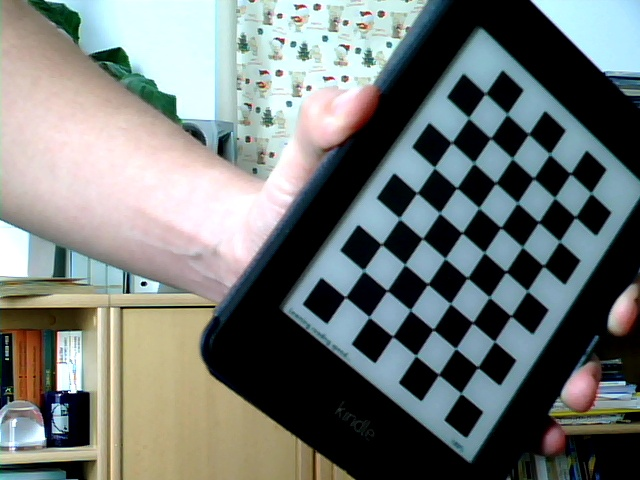
\includegraphics[width=160pt]{figures/left07.jpg}\hspace{10pt}
  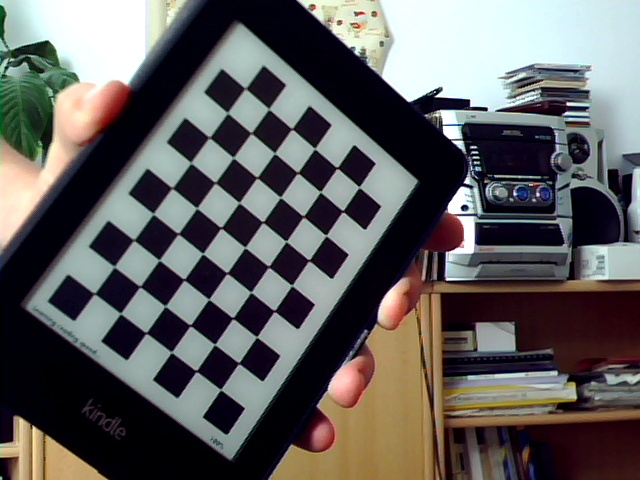
\includegraphics[width=160pt]{figures/right07.jpg}
  \caption{A kalibrációhoz felhasznált egyik képpár   \label{fig:stereo-calibration-before}}
\end{figure}

\begin{figure}[tbh]
  \centering
\begin{tikzpicture}[x=330,y=330]
	\node[anchor=south west,inner sep=0] at (0.515151,0) {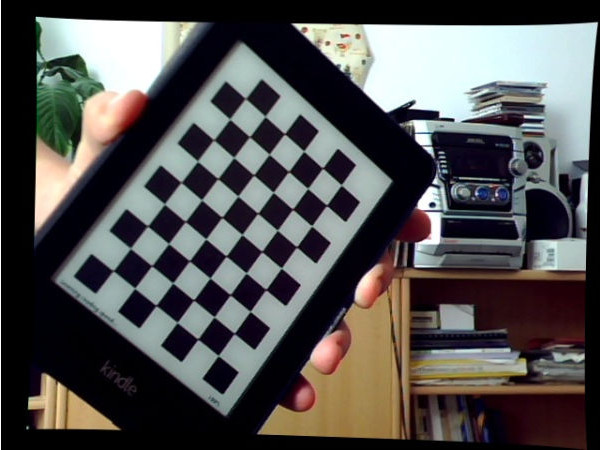
\includegraphics[width=160pt] {figures/calibrated_right.jpg}};
    \node[anchor=south west,inner sep=0] at (0,0) {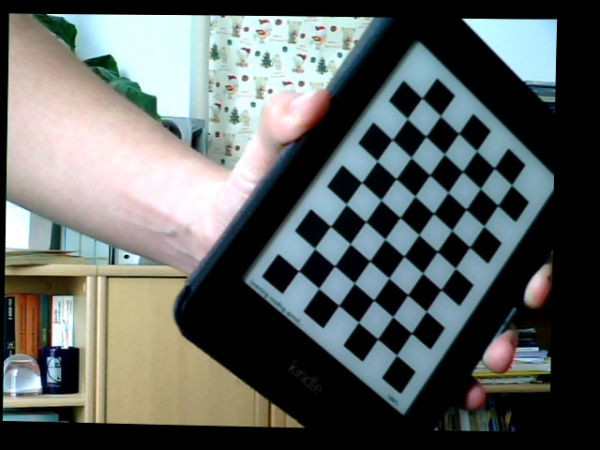
\includegraphics[width=160pt]    {figures/calibrated_left.jpg}};
    \draw[red,thick] (0,0.301) -- (1,0.301);
    \draw[red,thick] (0,0.200) -- (1,0.200);
    \draw[red,thick] (0,0.140) -- (1,0.140);
    \draw[red,thick] (0,0.045) -- (1,0.045);
\end{tikzpicture}
  \caption{Rektifikáció után a két kamera képe \label{fig:stereo-calibration-after}}
\end{figure}

\subsection{Optikai-folyam}

Az előzőekben megismert eljárás, azt feltételezi, hogy az egymásnak megfelelő pontok csak vízszintes irányban mozdulnak el, így, ha ezeket megtalálta, akkor az elmozdulás alapján már számolható mélységkép a kalibráció során felhasznált segéd-objektum alapján.

A most ismertetésre kerülő eljárás, az \textit{optikai-folyam}okat hívja segítségül, amelyekkel (mint elmozdulás vektorok) leírható, hogy adott pontok egymás utáni képkockákon hova mozdultak el. Ezt felhasználva nem szükséges a kamerákat párosával kalibrálni, sőt, már akár 1 kamerával is egy adott szilárd test lemodellezhető. Például tekintsük egy adott objektum felé néző mozgó kamera két helyzetében látott képet (lásd \aref{fig:triangulation}. ábrát). A kamerák pontjaiból az egyező képpontokba indított sugarak metszéspontjában (ami általában nem létezik, így Hartley és Zisserman \cite{HZ} ajánlását követve, a sugarakat összekötő legrövidebb szakasz középpontját választjuk) kereshető a való világbeli pont. Ezt \textit{háromszögeléses} módszernek hívjuk. Több egyező képpontot használva, ezen sugarak metszéspontait felírva megkaphatóak a pontok 3D-s koordinátái, valamint a két kamera közti transzformáció is kinyerhető. 

\begin{figure}[tbh]
\centering
\tdplotsetmaincoords{60}{130}
\begin{tikzpicture}[line join = round, line cap = round, >=triangle 45, tdplot_main_coords]
  
  \coordinate (O) at (0, 0, 0);
  
  % kocka
  
  \coordinate (C1) at (-4.5, -2, 1);
  \coordinate (C2) at (-4.5, -1, 1);
  \coordinate (C3) at (-4.5, -1, 2);
  \coordinate (C4) at (-4.5, -2, 2);
  \coordinate (C1B) at (-5, -2, 1);
  \coordinate (C2B) at (-5, -1, 1);
  \coordinate (C3B) at (-5, -1, 2);
  \coordinate (C4B) at (-5, -2, 2);
    \node [below right] at (C2) {\small $(X, Y, Z)$};

  \draw [dashed] (C1) -- (C2);
  \draw [dashed] (C2) -- (C3);
  \draw [dashed] (C3) -- (C4);
  \draw [dashed] (C4) -- (C1);
  \draw [dashed] (C1) -- (C1B);
  \draw [dashed] (C2) -- (C2B);
  \draw [dashed] (C3) -- (C3B);
  \draw [dashed] (C4) -- (C4B);
  \draw [dashed] (C1B) -- (C2B);
  \draw [dashed] (C2B) -- (C3B);
  \draw [dashed] (C3B) -- (C4B);
  \draw [dashed] (C4B) -- (C1B);
  
  
  % képsík
  
  \coordinate (I1) at (0, 0, 0);
  \coordinate (I2) at (0, 4, 0);
  \coordinate (I3) at (0, 4, 3);
  \coordinate (I4) at (0, 0, 3);

  \coordinate (_I1) at (-0.7, 5, 0);
  \coordinate (_I2) at (-0.7, 5, 3);
  \coordinate (_I3) at (-4.7, 5, 3);
  \coordinate (_I4) at (-4.7, 5, 0);


  \draw (I1) -- (I2);
  \draw (I2) -- (I3);
  \draw (I3) -- (I4);
  \draw (I4) -- (I1);
  
  \draw (_I1) -- (_I2);
  \draw (_I2) -- (_I3);
  \draw (_I3) -- (_I4);
  \draw (_I4) -- (_I1);

  \coordinate (UV) at (0, 0.421, 1.2368);
  \node [cross] at (UV) {};

  \coordinate (UV2) at (-3.5182, 5, 1.2727);
  \node [cross] at (UV2) {};

  % optikai tengely
  \coordinate (P1) at (0, 2, 1.5);
  \coordinate (C1) at (5, 2, 1.5);
  \coordinate (A1) at (-1, 2, 1.5);

  \coordinate (P2) at (-2.7, 5, 1.5);
  \coordinate (C2_) at (-2.7, 10, 1.5);
  \coordinate (A2) at (-2.7, 4, 1.5);

  \node [below] at (C1) {\small $C1$};
  \node [below] at (C2_) {\small $C2$};
  \draw (C1) -- (P1);
  \draw (C2_) -- (P2);
  \node [cross] at (P1) {};
  \node [cross] at (P2) {};
  \node [below right] at (P1) {\small $P1$};
  \node [below left] at (P2) {\small $P2$};
  \draw [dashed,-latex] (P1) -- (A1);
  \draw [dashed,-latex] (P2) -- (A2);
  
  % leképezés
  
  \draw [dotted] (C1) -- (C2);
  \draw [dotted] (C2_) -- (C2);
  
\end{tikzpicture}
\caption{Háromszögelés \label{fig:triangulation}}
\end{figure}

Optika-folyamok meghatározásánál a következő két fontos feltevéssel élünk:
\begin{itemize}
\item Az objektumokhoz tartozó képpontok intezitásai nem változnak képkockáról képkockára.
\item A szomszédos pontok elmozdulásai hasonlóak.
\end{itemize}

Meghatározásukra több algoritmus is létezik. Az egyik -- ami ritka vektor-mezőt generál jellegzetes pontok követéséhez -- a Lucas-Kanade \cite{LK} módszer (lásd \aref{fig:lk}. ábra). Ehhez szükséges először az, hogy az első képen a követendő pontokat (pl. Shi-Thomasi \cite{shi-thomasi} módszer által adott sarokpontok) azonosítsuk. Az LK módszer egy 9x9-es hálót definiál a pontok köré, és felteszi, hogy ezek elmozdulásai azonosak, és így oldja meg a már túl-határozott egyenletrendszert, hogy megkapjuk az elmozdulásvektorokat. Ez önmagában így csak kis mozgásokat tud követni, ezért nagy mozgások esetén a piramis-módszert használjuk; amikor is a képeket több lépcsőben kicsinyítjük, és ezeken is lefuttatjuk az algoritmusokat (ekkor a kis mozgások eltűnnek, a nagyok pedig kisebbekké válnak).

\begin{figure}[tbh]
\centering
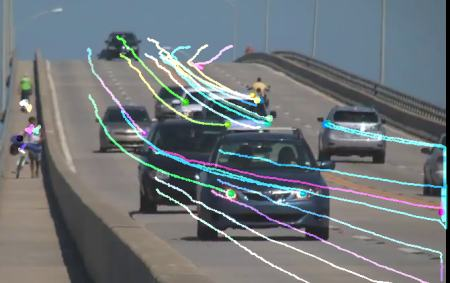
\includegraphics[width=300pt]{figures/opticalflow_lk.jpg}
\caption{Minta a sarokpontok követésére \cite{opencv-lk} \label{fig:lk}}
\end{figure}

A dolgozat során nekünk sűrű optikai-folyamok meghatározására lesz szükség, melyhez Gunner Farnebäck \cite{farneback} algoritmusát fogjuk használni. Ennek két praktikus haszna is van; egyrészt nem kell sarokpontokat keresnünk, másrészt pedig sűrű vektor-mezőt kapunk. \Aref{fig:dense-of}. ábrán látható egy példa, ami egy kanyon felett elrepülő helikopter videójának két egymás utáni képkockájából lett kiszámolva.

\begin{figure}[tbh]
\centering
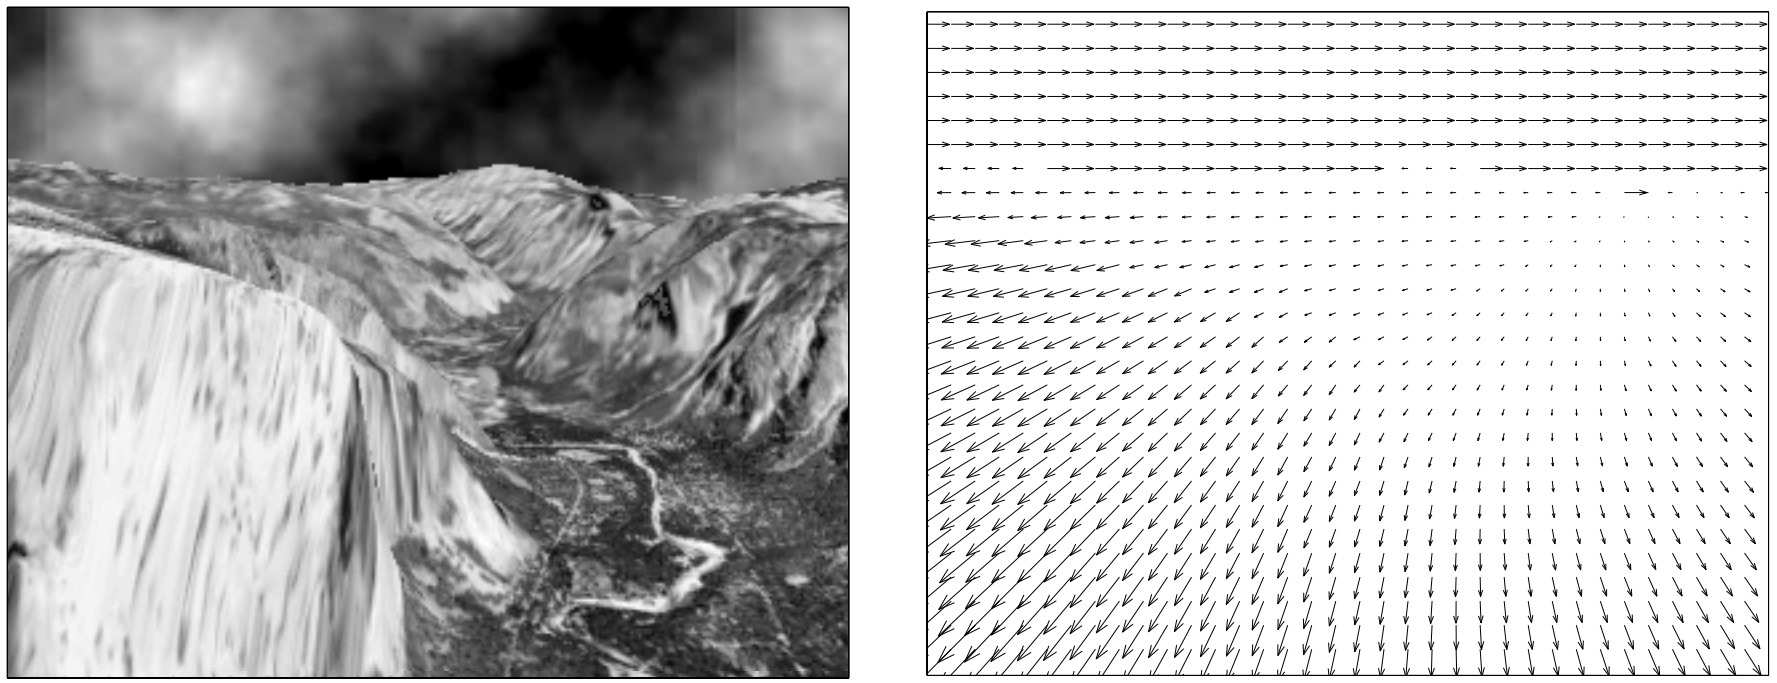
\includegraphics[width=420pt]{figures/farneback.png}
\caption{Minta sűrű optikai-folyam meghatározásra \cite{farneback} \label{fig:dense-of}}
\end{figure}

%----------------------------------------------------------------------------
\section{Objektum-detekció}
%----------------------------------------------------------------------------

A feladat megoldása során a mozgó objektumokat kell követnünk, azokat modellezni, így szükséges ezek detekciója.

Az előző részben leírt Farnebäck-módszert felhasználva kapunk egy becslést arra vonatkozóan, hogy hol lehetnek a mozgó tárgyak, hiszen a kamerák statikus helyzete révén, a háttér képpontjaihoz tartozóan 0 közeli elmozdulást várunk, míg a mozgó részeken ettől eltérőt.

Ezt kiegészíthetjük, egy háttér-előtér szegmentációs algoritmus felhasználásával \cite{MOG}, amely az egymás utáni képkockákból egy háttér-modellt épít, és így az aktuális képkockából azt kivonva, megkaphatjuk az éppen aktuális előtérhez tartozó maszkot, mintáért lásd \aref{fig:mog-example}. ábrát.

\begin{figure}[tbh]
\centering
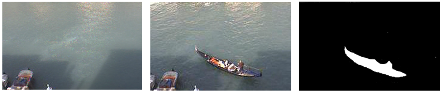
\includegraphics{figures/mog.png}
\caption{Minta a háttér-előtér elválasztási algoritmus eredményére \cite{mog-example} \label{fig:mog-example}}
\end{figure}

A maszkot és a vektor-mezőt felhasználva, már igen jó közelítéssel megkaphatjuk a mozgó objektumoknak megfelelő képszeleteket.
